\documentclass[%
aip,
amsmath,amssymb,
reprint,%
% Conference Proceedings
]{revtex4-1}

\usepackage{graphicx}% Include figure files
\usepackage{dcolumn}% Align table columns on decimal point
\usepackage{bm}% bold math

\usepackage[utf8]{inputenc}
\usepackage[T1]{fontenc}
\usepackage{mathptmx}
\usepackage{graphicx}
\usepackage{array}
\usepackage{listings}
\usepackage{color}

\definecolor{codegreen}{rgb}{0,0.6,0}
\definecolor{codegray}{rgb}{0.5,0.5,0.5}
\definecolor{codepurple}{rgb}{0.58,0,0.82}
\definecolor{backcolour}{rgb}{0.95,0.95,0.92}
 
\lstdefinestyle{mystyle}{
    backgroundcolor=\color{backcolour},   
    commentstyle=\color{codegreen},
    keywordstyle=\color{magenta},
    numberstyle=\tiny\color{codegray},
    stringstyle=\color{codepurple},
    basicstyle=\footnotesize,
    breakatwhitespace=false,         
    breaklines=true,                 
    captionpos=b,                    
    keepspaces=true,                 
    numbers=left,                    
    numbersep=5pt,                  
    showspaces=false,                
    showstringspaces=false,
    showtabs=false,                  
    tabsize=2
}
\lstset{style=mystyle}


\begin{document}

\title{Detecting Expolanets using Unsupervised Deep Learning}

\author{Naveen Mathew Nathan Sathiyanathan}
\affiliation{Department of Statistics, University of Illinois at Urbana-Champaign}

\date{\today}

\begin{abstract}
Exoplanet detection using transit method is currently a manual process. It involves identification of clear troughs in the intensity of light for a sustained period. Previous works have tried to automate the process using BLS (Box-fitting Least Squares) and TLS (Transit Least Squares). Supervised machine learning algorithms such as CNN, wavelet MLP, SVM and Bayesian MCMC have been applied with varying levels of success. The objective of this paper is not to improve on these methods, but to open doors for unsupervised methods in exoplanet detection. The report concludes with examples of true positives and false positives and mentions ways to improve the performance.
\end{abstract}

\maketitle

\section{Introduction}

The first exoplanet was discoveed in 1995. The rate of discovery of exoplanets has increased over the years. Kepler was the first space telescope that scanned for exoplanets. Nowadays there are other telescopes such as KELT, HATNet, CoRoT, TESS (future), Plato (future) and LSST (future). As a result, manual identification becomes tedious. The required manpower is often not available to perform this task.

Several attempts were made to automate the process of detecting troughs in light curve. These include methods that use classical statistics, time series analysis. Recently several machine learning solutions have been used and have shown promising results. All available solutions are supervised. Therefore, they tend to exhibit the same biases as humans. An unsupervised method was explored for exoplanet identification using light curves which was expected to involve fewer human biases. Specifically, LSTM autoencoder was used to compress the available information and to identify anomalous patterns - such as eclipsing binary stars or exoplanets.

\section{Literature Survey}

Various statistical learning algorithms have been applied to the problem of exoplanet detection using transit method. BLS (Box-fitting Least Squares) described by Kovacs et al. (2016). The algorithm searches for signals characterized by a periodic alternation between two discrete levels, with much less time spent at the lower level. They apply several transormations on the data to compute useful metrics. Firstly they compute Signal Detection Efficiency: $SDE = \frac{SR_{peak}-<SR>}{sd(SR)}$ and use $\alpha = \frac{\delta}{\sigma}\sqrt{nq}$ to parameterize the effective SNR (signal-to-noise ratio). They performed several simulations and observed that the model performed better than previous works even at low SNR.

Pearson et al. (2017) discussed the use of neural networks for exoplanet detection using light curves. They setup the task as a supervised binary classification problem and used methods such as MLP, wavelet MLP, SVM and CNN to model the light curve. They observed that wavelet MLP and CNN had similar ROC curves, but CNN led to better separation as it had lower loss function value after training. They also observed that CNN performs significantly better than other algorithms at low resolutions and that the difference decreases with increase in resolution. They also found that the performance improved after phase folding.

Christopher et al. (2018) applied logistic regression, fully connected feed forward network and CNN with pooling on human tagged transit data to predict planetary transits from light curves. They applied different types of data augmentation to create artificial data from manually labelled observations. They also used three different inputs - global, local and both - to classify the light curve image. Google Vizier was used for hyperparemeter tuning. Finally, the models were averaged to reduce the error rate. Using this method they were able to identify 2 new candidates that were later confirmed as exoplanets.

Chong et al. (2017) applied a spatiotemporal architecture for anomaly detection in videos. The architecture included two components: one for spatial feature representation and one for learning temporal evolution of spatial features. Through experiments they found that the results were comparable to state-of-the-art methods and was considerably faster - therefore it supported videos with higher frame rates.

Marchi et al. (2015) applied bidirectional LSTM (denoising) autoencoder in unsupervised setting to detect anomalous behavior in acoustic signals. They used the reconstruction error to detect anomalies. The autoencoder was trained on a public dataset of recordings of in-hom situations such as talking, watching television, playing and eating. The model achieved up to 0.934 F-measure, which significantly outperformed state-of-the-art methods.

Malhotra et al. (2016) applied LSTM autoencoder for anomaly detection in signals from multiple detectors. The conducted the experiment on three public data sets: power demand, space shuttle and ECG; and two real-world engine data sets. They observed that the LSTM autoencoder was robust in predictable, unpredictable, periodic, aperiodic and quasi-peridic time series. They also observed that the model was able to detect anomalies in short time series as well as long time series.

These efforts all involve supervised machine learning. They incorporate human biases in the output variable. Therefore, the patterns they learn contain human biases. The objective of this project is to use anomaly detection to flag different types of patterns - not limited to planetary transits.

\section{Data Description}

Kepler contains several forms of light curve data. For this project Kepler KOI DV data set was chosen. The expected size was around 100 GB. Only a 25 GB subset was downloaded for convenience. The downloaded data contains 3050 files. Each file consists of time series and covers Q1-Q16.

The downloaded files contain data from 2205 stars. Each star has at least one orbiting planet. Distribution of number of planets around the stars is given below:

\begin{center}
 \begin{tabular}{| c | c |} 
 \hline
 \textbf{Number of Planets} & \textbf{Count of Stars}\\ [0.5 ex]
 \hline
 1 & 1595 \\ 
 \hline
 2 & 454 \\
 \hline
 3 & 105 \\
 \hline
 4 & 33 \\
 \hline
 5 & 11 \\
 \hline
 6 & 5 \\
 \hline
 7 & 1 \\
 \hline
 8 & 1 \\
 \hline
 \textbf{Total} & \textbf{2205} \\ [1ex] 
 \hline
\end{tabular}
\end{center}


\subsection{Variables}

Data description provided in Kepler page \footnote{Link: https://exoplanetarchive.ipac.caltech.edu/docs/KeplerDV.html}:

\begin{itemize}
  \item TIME: Time in seconds after Barycentric Kepler Julian Date (BKJD = BJD - 2454833).
  \item CADENCE\_NUMBER: A measure of (time) resolution of observations.
  \item INIT\_FLUX\_PL: Unfilled, normalized, harmonic-removed input to planet search algorithm for this TCE. Previously identified TCEs have been gapped.
  \item INIT\_FLUX\_PL\_ERR: Uncertainty in the initial flux.
  \item MODEL\_LC\_PL: Filled, normalized model light curve calculated from the planetary fit to the TCE.
  \item RESIDUAL\_FLUX: INIT\_FLUX\_LAST\_PLANET with model transits gapped – median(INIT\_FLUX\_LAST\_PLANET with model transits gapped).
  \item RESIDUAL\_FLUX\_ERR: Uncertainty in the residual flux.
\end{itemize}

\section{Exploratory Analysis}

Summary statistics of the number of planets around each star:

\begin{center}
 \begin{tabular}{| c | c |} 
 \hline
 \textbf{Statistic} & \textbf{Value}\\ [0.5 ex]
 \hline
 Mean & 1.383 \\ 
 \hline
 Median & 1 \\
 \hline
 Mode & 1 \\
 \hline
 Standard deviation & 0.748 \\
 \hline
 Range & [1, 8] \\
 \hline
 Q1 & 1 \\
 \hline
 Q3 & 2 \\ [1ex] 
 \hline
 \end{tabular}
\end{center}

For simplicity, only RESIDUAL\_FLUX column was considered for analysis. The residual flux column comprises of the following components:

\begin{itemize}
  \item Trend in mean brightness of host star.
  \item Changes in brightness due to orbiting planets, asteroids, comets and debris.
\end{itemize}

Since the median was subtracted, for a non-variable star, the residual flux is almost a pure Gaussian noise with constant variance. However, in presence of a planetary transit, the light curve shows significant deviation from the noisy process. Therefore, the joint multivariate distribution of consecutive observations is expected to shift significantly in presence of exoplanets.


\begin{figure}[h!]
	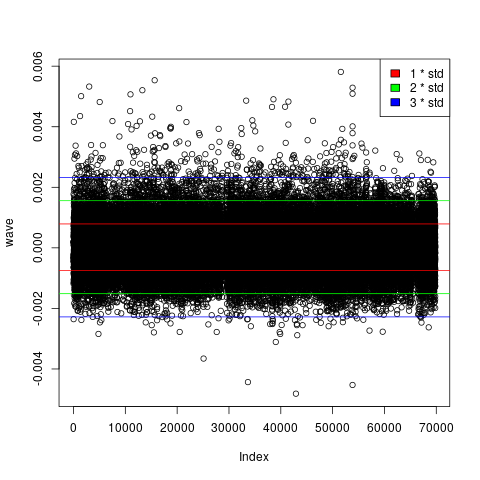
\includegraphics[width=\linewidth]{example.png}
	\caption{Residual Flux vs Time.}
	\label{fig:res_flux}
\end{figure}

Based on these observations, it is not possible to analyze the flux as a simple stationary Gaussian noise without a processes that drives the variation in flux. Thresholds such as $mean \pm 3 \times stdev$ will lead to large number of false positives.

\section{Preprocessing}

\subsection{Capping}

From the above plot it was observed that the flux shows unusual variations above the 3 standard deviation mark. This can be because of several reasons such as increase in intensity of the star over time or due to environmental factors that inflence the noise. To minimize the effect of this noise, values of residual flux were capped at 97.5 percentile. However, systematic variations that lead to increased flux will lead to significant difference in representation at the bottleneck layer.

\subsection{Imputing Missing Values}

The data is in time series format with missing values. Training a network is not possible in presence of missing values. Since the missing values are clustered together, the process of imputing values becomes difficult. A method called Stineman interpolation was used to fill the missing values of residual flux. This smooths the residual flux during the missing period.

\section{Modeling}

Under the assumption of stationarity, the expected proportion of observations outside $mean \pm 3 \times stdev$ is 0.0027. However, despite the near normality of the distribution, the observed proportion is much higher. In such cases it is uncertain whether there are orbiting planets or debris around the host star. Humans can detect orbiting exoplanets only when there is a significant shift in the light curve.

$$\mu_{seqlen} = f(\mu_{seqlen-1,seqlen-2, ...}) + \epsilon; \epsilon \sim N(0, \sigma^2)$$

If the distribution of flux is modeled based on a series of finite number of previous values of flux, under the assumption of normality of flux, the squared error is expected to have a chi-square distribution. However, any shift in light curve will be characterized by a high value of squared reconstruction error.

\subsection{Phase Folding}

Phase folding is a technique used in time series, especially in analysis of astronomy time series data. The purpose is to superimpose signals to get a smoothed time series that exhibits lesser noise and more signal. Therefore, the signal-noise ratio is enhanced. This is achieved by plotting the signal vs phase.

Phase folding was done using a simple idea: if the periodicity is correctly identified, the standard deviations of the series at the time slices will be approximately equal. For obtaining periodicity it was assumed that the signal repeats itself at least twice (excluding imputed values). The following steps were used:

\begin{itemize}
\item Initialize a lower and upper bound for periodicity
\item While upper bound > lower bound
\begin{itemize}
\item Calculate $half\_width = \frac{upper-lower}{2}$, $mid = lower + half\_width$
\item Create chunks of width equal to lower/mid/upper bound
\item Calculate ratio of maximum to minimum standard deviation
\item If ratio is smaller for lower bound
\begin{itemize}
\item Set lower := lower - half\_width, upper := mid
\end{itemize}
\item If ratio is smaller for mid bound
\begin{itemize}
\item Set lower := lower + half\_width/2, upper := upper - half\_width/2
\end{itemize}
\item If ratio is smaller for upper bound
\begin{itemize}
\item Set lower := mid, upper := upper + half\_width
\end{itemize}
\item If all ratios are equal
\begin{itemize}
\item Do not update lower and upper
\item Exit loop
\end{itemize}
\end{itemize}
\item Return values: lower and upper
\end{itemize}

\subsection{Autoencoder}

An autoencoder is used to model the (joint) distribution of one or more variables. An autoencoder attempts to reconstruct the original signal from the input by passing it through information bottleneck. The amount of details retained in the representation on input at the bottleneck depends on the number of units in the bottleneck. If the structure of the network is fixed from the input to bottleneck, the reconstruction error at the output cannot be decreased below a minimum threshold that is determined by the amount of information at the bottleneck.

\subsection{LSTM}

Several models of memory have been proposed in the past. These models explicitly use finite (such as Markov model) or infinite number (such as exponential weights) of past states as memory. Long short term memory (LSTM) were proposed to model memory in neural networks. LSTM autoencoders have been applied successfully in industrial IoT for anomaly detection in time series data. This makes them suitable for anomaly detection in light curves.

\begin{figure}[h!]
	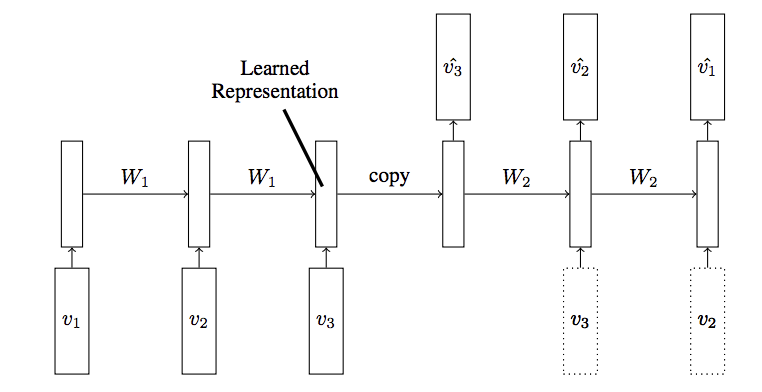
\includegraphics[width=\linewidth]{LSTM-Autoencoder-Model.png}
	\caption{Standard LSTM Autoencoder.}
	\label{fig:lstm_autoenc}
\end{figure}

\subsection{Hyper-Parameters}

There are several tunable hyperparameters in the model. The following combination of hyperparameters were used:

\begin{itemize}
  \item Sequence length: 10.
  \item Number of LSTM layer(s): 3.
  \item LSTM activation(s):
  \begin{itemize}
      \item Activation: tanh.
      \item Recurrent activation: hard sigmoid.
  \end{itemize}
  \item Number of units in each LSTM layer(s): 64, 256, 100.
  \item Recurrent droupout: 0.2, 0.2, 0.2.
  \item Number of dense layer(s): 1.
  \item Number of units in dense layer(s): 1.
  \item Activation(s) of dense layer(s): Linear.
  \item Loss function: Mean squared error.
  \item Optimization scheme: Adam (learning rate = 0.1).
  \item Batch size: 50
  \item Number of epochs: 10
\end{itemize}

\subsection{Learning}

The process of learning starts with random initializations of the weights in recurrent and dense layers. A mini batch of size 50 was used to compute the estimate of MSE and its gradient with respect to the parameters. The overall training was run for 10 epochs because the interpreter was unable to perform early stopping based on validation loss. Adam optimization scheme was used to find the minimizer. An example learning curve can be found below:

\begin{figure}[h!]
	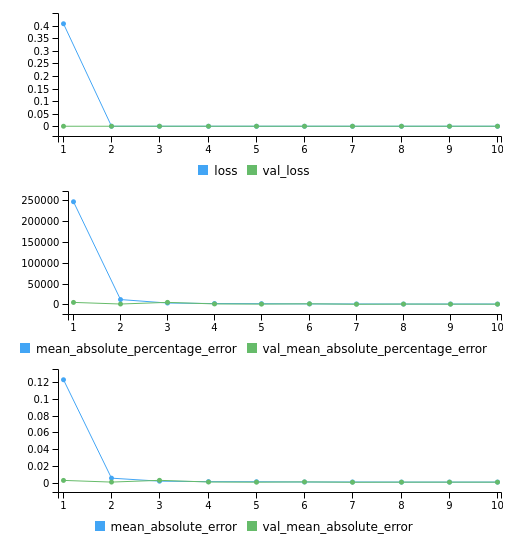
\includegraphics[width=\linewidth]{learning.png}
	\caption{Learning Curve.}
	\label{fig:learning}
\end{figure}

Based on the learning curves obtained from the 34 files it was concluded that the process of learning has occurred reasonably well in 10 epochs. Almost all fits show that the training loss, MAE and MAPE are close to the validation loss, APE and MAPE respectively. Therefore, the fitted models are appropriate for prediction.

\section{Results and Conclusions}

\begin{center}
 \begin{tabular}{|c | c | c | c |} 
 \hline
 \textbf{Dataset} & \textbf{Metric} & \textbf{Value - Train} & \textbf{Value - Validation} \\ [0.5 ex]
 \hline
 003732821 & Loss & $2.310446 \times 10^{-7}$ & $2.312617 \times 10^{-7}$ \\ 
 \hline
 003732821 & MAPE & 118.83902 & 125.8919 \\
 \hline
 003732821 & MAE & $3.867701 \times 10^{-4}$ & $3.769676 \times 10^{-4}$ \\
 \hline
 010790387 & Loss & $1.509265 \times 10^{-7}$ & $1.466977 \times 10^{-7}$ \\ 
 \hline
 010790387 & MAPE & 230.77675 & 121.3132 \\
 \hline
 010790387 & MAE & $3.075688 \times 10^{-4}$ & $3.081162 \times 10^{-4}$ \\
 \hline
 010879213 & Loss & $9.718002 \times 10^{-6}$ & $7.469951 \times 10^{-4}$ \\ 
 \hline
 010879213 & MAPE & 38.79628 & 403.0349 \\
 \hline
 010879213 & MAE & $2.484605 \times 10^{-3}$ & $2.00089626 \times 10^{-2}$ \\
 \hline
 010155029 & Loss & $6.862203 \times 10^{-8}$ & $3.177653 \times 10^{-8}$ \\ 
 \hline
 010155029 & MAPE & 198.06549 & 138.9201 \\
 \hline
 010155029 & MAE & $9.513334 \times 10^{-5}$ & $1.398749 \times 10^{-4}$ \\
 \hline
 001995732 & Loss & $8.851227 \times 10^{-7}$ & $8.462837 \times 10^{-7}$ \\ 
 \hline
 001995732 & MAPE & 210.76816 & 141.6288 \\
 \hline
 001995732 & MAE & $7.366635 \times 10^{-4}$ & $7.207151 \times 10^{-4}$ \\[1ex] 
 \hline
\end{tabular}
\end{center}

\subsection{Plots}

\begin{figure}[h!]
	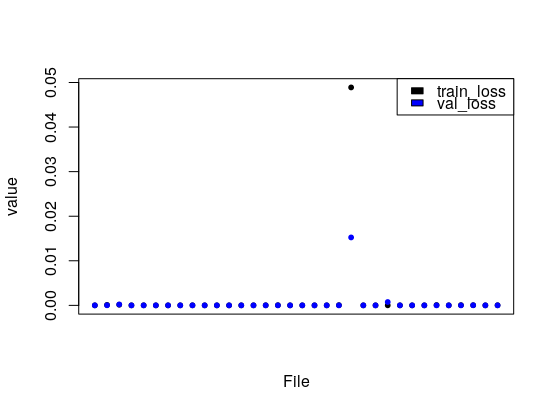
\includegraphics[width=\linewidth]{loss.png}
	\caption{Loss Comparison.}
	\label{fig:loss}
\end{figure}

\begin{figure}[h!]
	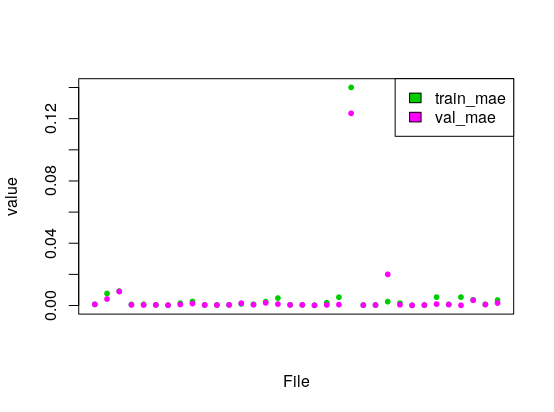
\includegraphics[width=\linewidth]{mae.png}
	\caption{MAE Comparison.}
	\label{fig:mae}
\end{figure}

\begin{figure}[h!]
	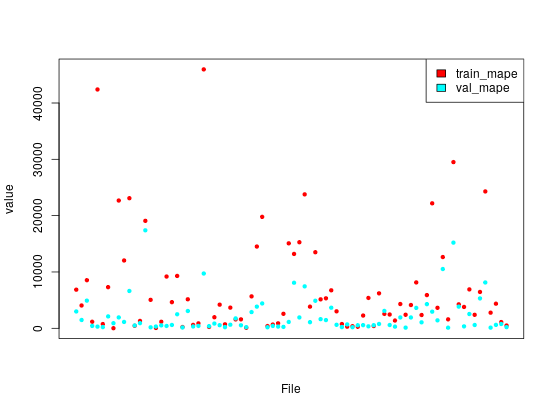
\includegraphics[width=\linewidth]{mape.png}
	\caption{MAPE Comparison.}
	\label{fig:mape}
\end{figure}

\begin{figure}[h!]
	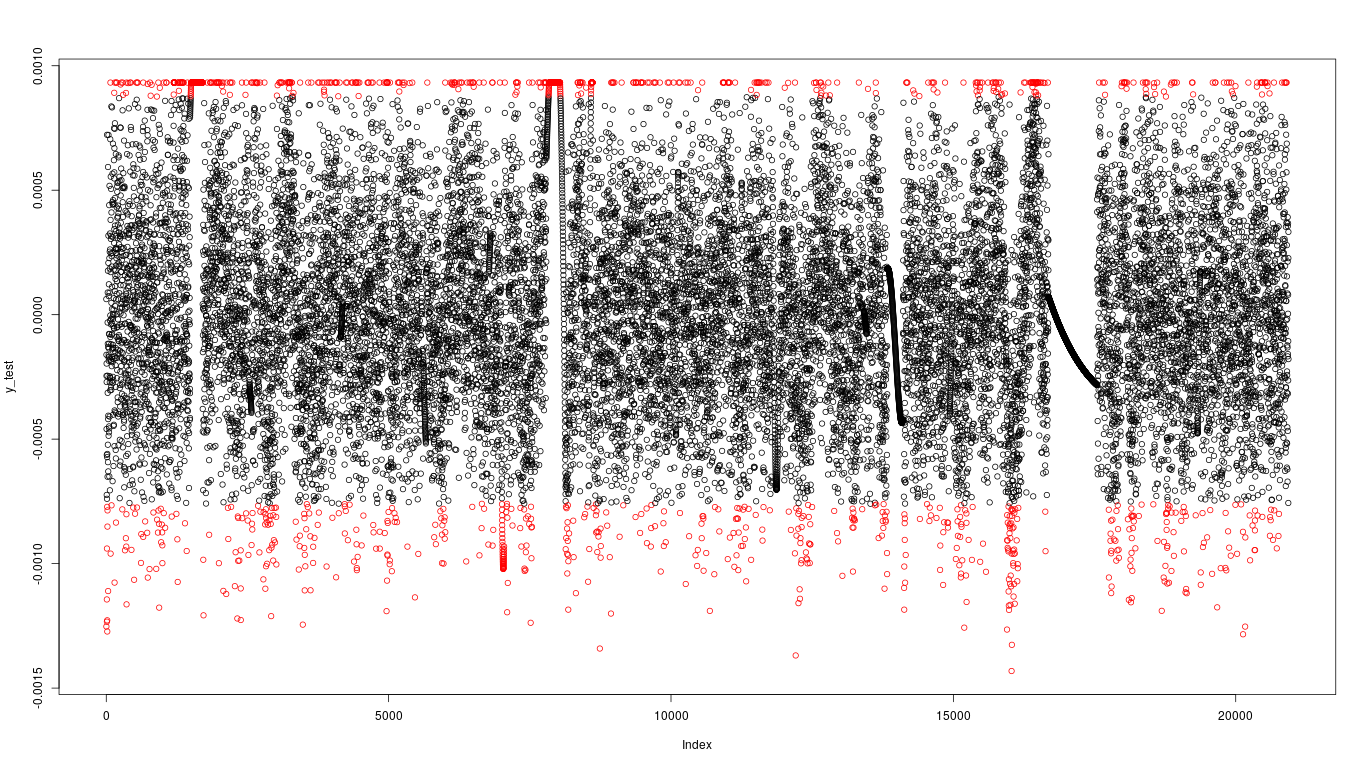
\includegraphics[width=\linewidth]{eg1_before.png}
	\caption{Example detection - before phase folding}
	\label{fig:eg1_before}
\end{figure}

\begin{figure}[h!]
	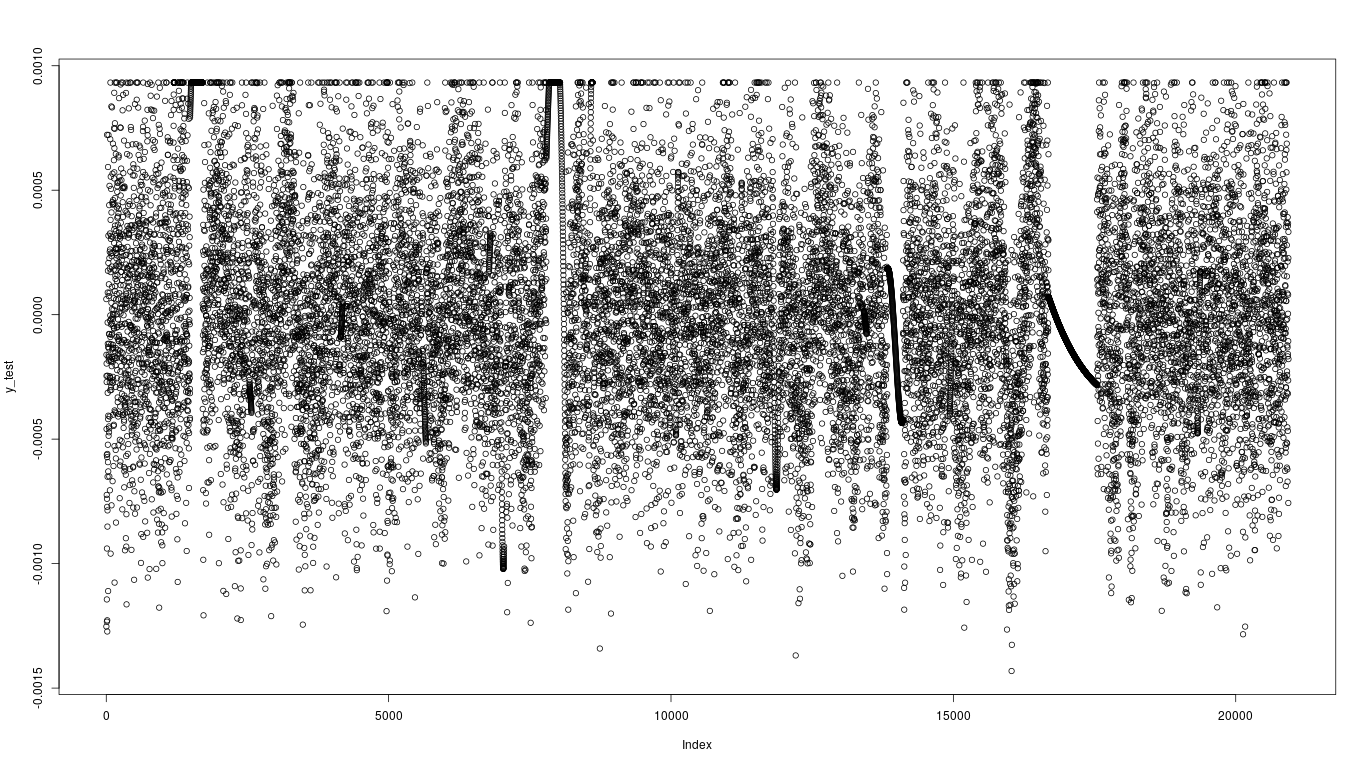
\includegraphics[width=\linewidth]{eg1_after.png}
	\caption{Example detection - after phase folding}
	\label{fig:eg1_after}
\end{figure}

\begin{figure}[h!]
	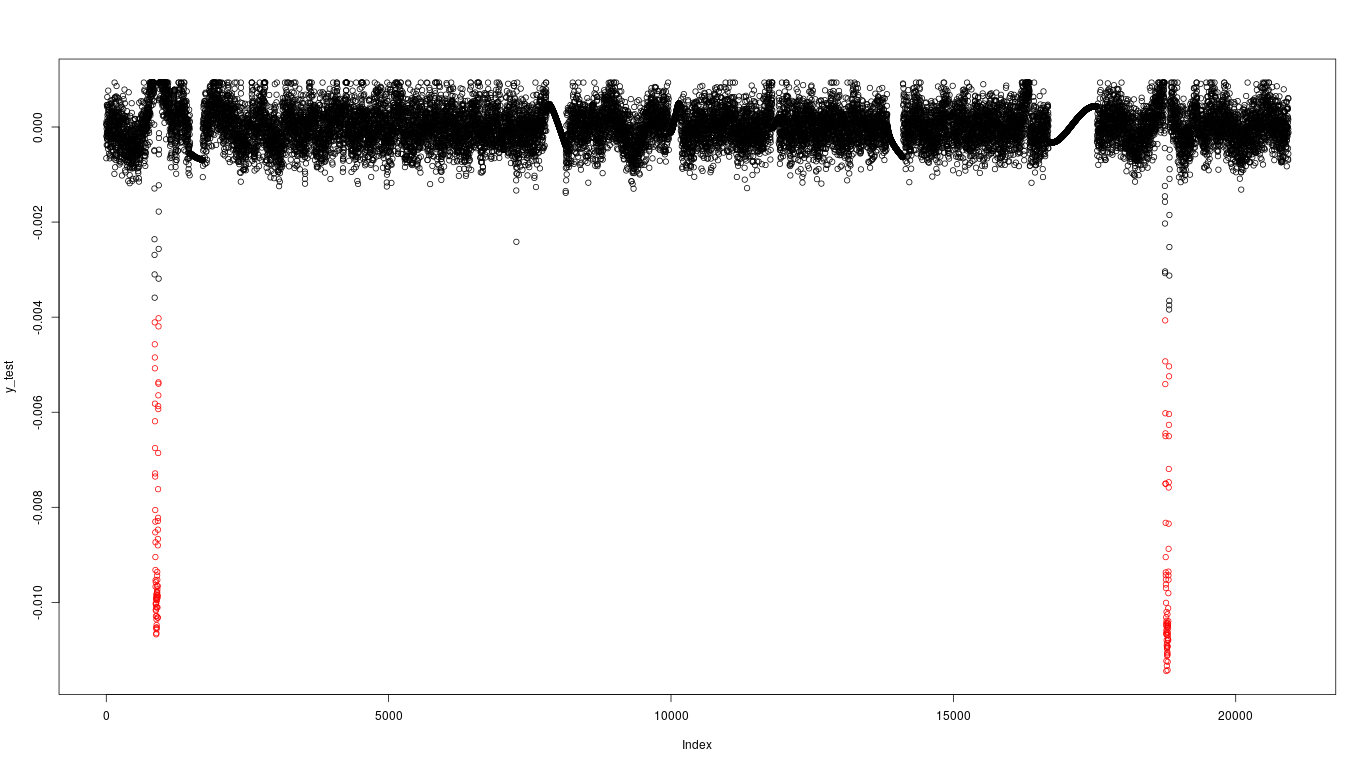
\includegraphics[width=\linewidth]{eg2_before.png}
	\caption{Example detection - before phase folding}
	\label{fig:eg2_before}
\end{figure}

\begin{figure}[h!]
	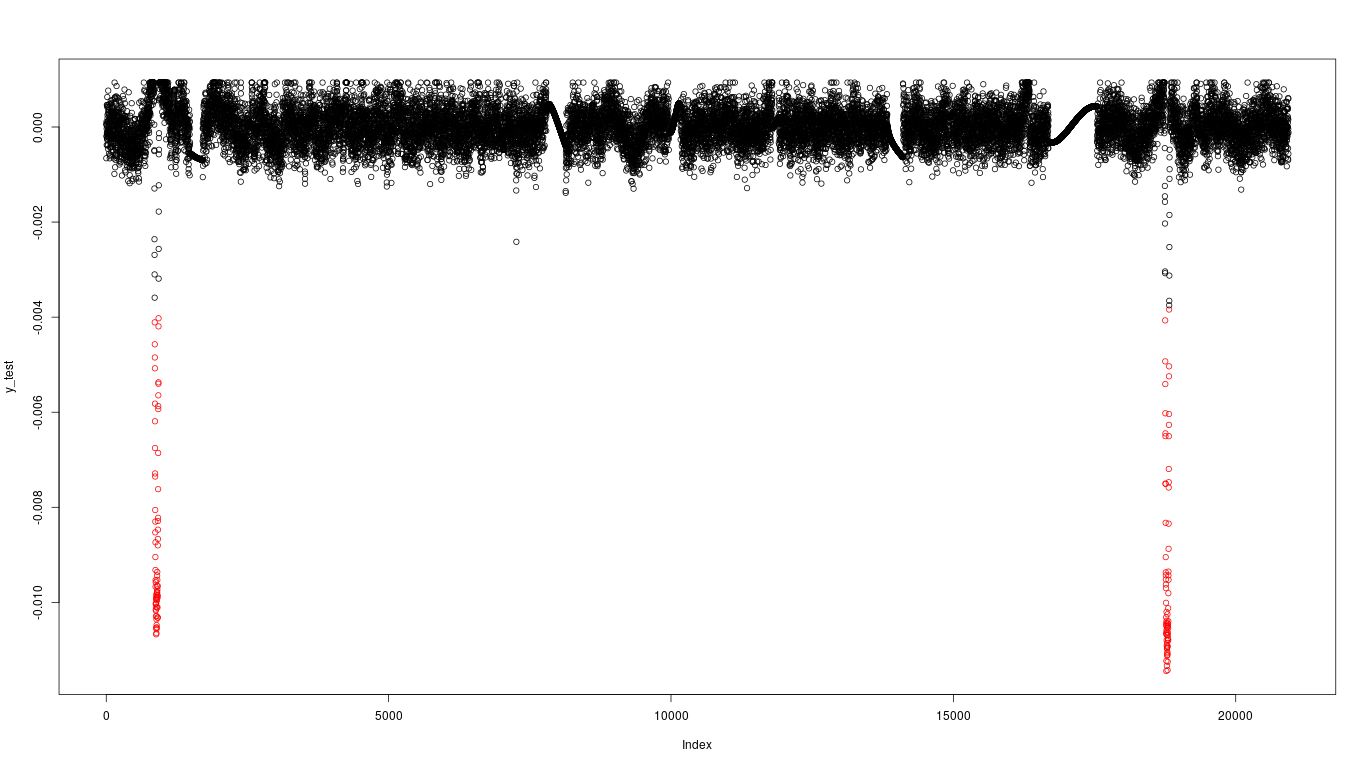
\includegraphics[width=\linewidth]{eg2_after.png}
	\caption{Example detection - after phase folding}
	\label{fig:eg2_after}
\end{figure}

\section{Scope for Improvement}

The assumptions used in the model create artificial constraints on the patterns learnt by the autoencoder. Firstly, the directionality of memory leads to unusual performance during planetary transits. Since planetary transits occur over a period that is usually longer than the sequence length, incorporating bidirectional memory (past and future) can improve the detection rate. This can be done by using a bidirectional LSTM autoencoder. The resulting model can be written as:

$$\mu_{seqlen} = f(\mu_{seqlen-1,seqlen-2, ..., seqlen+1, seqlen+2, ...}) + \epsilon; \epsilon \sim N(0, \sigma^2)$$

The model hyperparameters were fixed during training due to time constraints (only 3 hours for training and prediction). These hyperparameters can vary significantly for different types of transits (duration, latitude of entry, eccentricity and orientation of orbit around the star). Hyperparameter tuning using tfruns is recommended.

Lastly, cases of anomalies above the mean were not explicitly excluded. This was done intentionally to avoid introducing human bias into the model - anomalous increase in star brightness is also an interesting astronomical event that may require scrutiny. Explicit removal of these detections can lead to better exoplanet transit detection.

\vspace{140 mm}
\section*{Appendix}

\subsection{Code Samples}

\begin{itemize}
\item Preprocessing
\end{itemize}

\lstinputlisting[language=R, firstline=64, lastline=77]{"../main.R"}

\begin{itemize}
\item Model building
\end{itemize}

\lstinputlisting[language=R, firstline=158, lastline=160]{"../main.R"}
\lstinputlisting[language=R, firstline=200, lastline=218]{"../main.R"}

\begin{itemize}
\item Phase folding
\end{itemize}

\lstinputlisting[language=R, firstline=15, lastline=62]{"../main.R"}


\subsection{References}
\begin{itemize}
\item Kepler KOI DV bulk data downloader \footnote{Link: https://exoplanetarchive.ipac.caltech.edu/bulk\_data\_download/\\Kepler\_KOI\_DV\_wget.bat}
\item A box-fitting algorithm in the search for periodic transits (Kovács et al., 2002)
\item Identifying Exoplanets with Deep Learning: A Five Planet Resonant Chain around Kepler-80 and an Eighth Planet around Kepler-90 (Christopher J. Shallue and Andrew Vanderburg, 2018)
\item Machine-learning Approaches to Exoplanet Transit Detection and Candidate Validation in Wide-field Ground-based Surveys (Schanche et al., 2018)
\item Abnormal Event Detection in Videos using Spatiotemporal Autoencoder (Chong et al., 2017)
\item A novel approach for automatic acoustic novelty detection using a denoising autoencoder with bidirectional LSTM neural networks (Marchi et al., 2015)
\item LSTM-based Encoder-Decoder for Multi-sensor Anomaly Detection (Malhotra et al., 2016)
\end{itemize}



\end{document}
